Une entreprise peut produire entre 0 et $40$ tonnes de compote par mois.

Le coût de production de $x$ tonnes de compote, exprimé en euros, est donné par la fonction $C$ définie sur $[0~;~40]$.

La recette réalisée pour $x$ tonnes de compote vendues, exprimée en euros, est donnée par la fonction $R$ définie sur $[0~;~40]$.

Dans cet exercice on s'intéresse à la différence entre la recette et le coût de production. Lorsque cette différence est positive on l'appelle le bénéfice.

\subsection*{Partie A -- Étude graphique}

Les représentations graphiques $\mathcal{C}_C$ et $\mathcal{C}_R$ des fonctions $C$ et $R$ sont données ci-dessous.

\begin{center}
	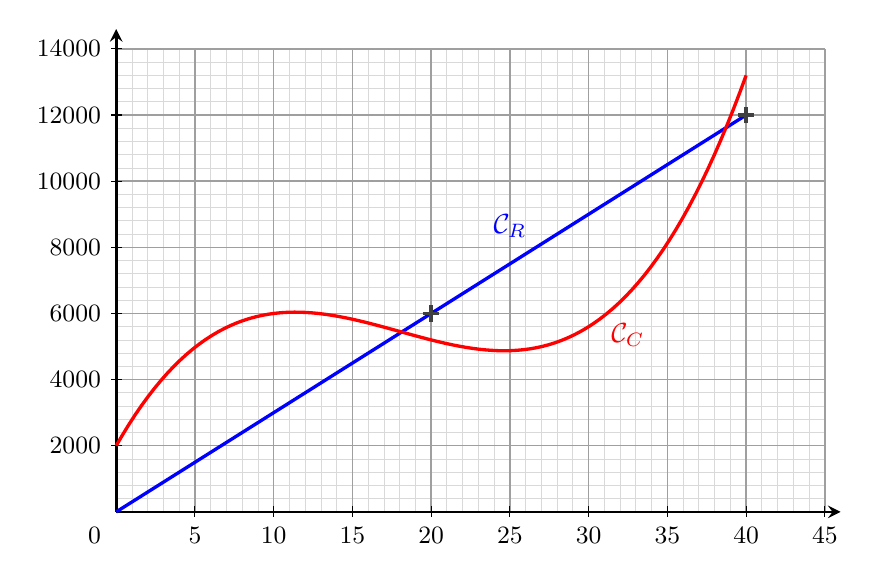
\begin{tikzpicture}[x=0.2cm,y=0.42cm,>=stealth]
		
		\draw[xstep=1,ystep=0.4,gray!30,line width=0.3pt] (0,0) grid (45,14);
		\draw[xstep=5,ystep=2,gray!75,line width=0.5pt] (0,0) grid (45,14);
		\draw[->,line width=1pt] (0,0) -- (46,0);
		\draw[->,line width=1pt] (0,0) -- (0,14.6);
		\foreach \x in {5,10,...,45} \draw (\x,2pt) -- (\x,-2pt) node[below] {\small \x};
		\foreach \y in {2,4,...,14} \draw (2pt,\y) -- (-2pt,\y) node[left] {\small \np{\y000}};
		\draw (-2pt,-2pt) node[below left] {\small 0};
		\draw[line width=1.2pt,blue] plot[domain=0:40] (\x,{0.3*\x});
		\draw[line width=1.2pt,red] plot[domain=0:40,samples=100] (\x,{(\x/10)^3-5.4*(\x/10)^2+8.4*(\x/10)+2});
		\foreach \P in {(20,6),(40,12)} \draw[line width=1.25pt,darkgray,shift={\P}] (-3pt,0) -- (3pt,0) (0,-3pt) -- (0,3pt);
		\node[red,below] at (32.5,6) {$\mathcal{C}_C$};
		\node[blue,above] at (25,8) {$\mathcal{C}_R$};
	\end{tikzpicture}
\end{center}

Vous répondrez aux trois questions suivantes en vous appuyant uniquement sur ce graphique.

\begin{enumerate}
	\item Déterminer l'expression $R(x)$ de la recette réalisée pour $x$ tonnes de compote vendues.
	\item Pour quelle(s) valeur(s) de $x$ l'entreprise réalise-t-elle un bénéfice ? On donnera des valeurs approchées à l'entier près.
	\item Avec la précision permise par le graphique, évaluer le bénéfice maximal réalisé par l'entreprise.
\end{enumerate}

\subsection*{Partie B -- Étude du résultat}

On admet que le résultat réalisé pour $x$ tonnes de compote fabriquées et vendues, exprimé en euro, est donné par la fonction $B$ définie sur l'intervalle $[0~;~40]$ par :
\[ B(x) = -x^3+54x^2-540x-\np{2000} \]

On donne les valeurs suivantes :
\[B(0) = -\np{2000} \,;\quad B(6) = -\np{3512} \,;\quad B(30) = \np{3400} \,;\quad B(40) = -\np{1200}\]

\begin{enumerate}
	\item On note $B'$ la fonction dérivée de la fonction $B$.

	Calculer $B'(x)$ et montrer que $B'(x)$ peut s'écrire sous la forme :
	\[ B'(x) = (-3x + 18)(x - 30) \]
	\item Étudier le signe de $B'$ sur l'intervalle $[0~;~40]$ et en déduire les variations de la fonction $B$ sur ce même intervalle.
	\item Pour quelle quantité de compote le bénéfice réalisé par l'entreprise est-il maximal ?
\end{enumerate}

\medskip
